\chapter{Prelogomena}
\label{ch:general-preliminaries}

\begin{chapterpresentation}
	\begin{abstract}
		We introduce the basic definitions and notations used throughout this thesis.
		Rather than reading it linearly, we recommand to skim it
		to get an idea of what it contains, and to only go back to this chapter
		only when needed, using the numerous internal hyperlinks.
	\end{abstract}
		
	\par\bigskip\bigskip
	\chaptertoc
\end{chapterpresentation}

\paragraph*{Notations.}
We try to use notations that syntactically reflect their type:
for instance, given a set $X$, we use Roman lowercases ($x,y,z,\dotsc$)
to denote elements of $X$, Roman uppercases for its subsets ($A, B, C, \dotsc$),
and cursive letters ($\+X, \dotsc$) for sets of subsets of $X$.
Functions are denoted by $f, g, h$, etc. and relations by
uppercase cursive letters ($\+R, \+S, \dotsc$).

Tuples $\tup{x_1,\dotsc,x_k}$ are sometimes denoted by $\bar x$.
Machines (Turing machines, automata, etc.) are also denoted
with uppercase cursive letters ($\+T$, $\+A$, $\dotsc$).
On the other hand, Greek letters are used to either denote queries ($\gamma, \delta, \dotsc$),
formulas ($\phi, \chi, \psi, \dotsc$) or monoid morphisms ($\phi, \chi, \psi, \eta$). When possible, we try to
use the letter to recall the semantics of the object: for instance in
\Cref{ch:semantic-tree-width-CRPQ}, $\gamma$ will be used to denote a base query,
$\alpha$ for one of its "\textbf{a}pproximation@approximation",
$\rho$ for a "\textbf{r}efinements@refinement" and
$\chi$ for an "e\textbf{x}pansion@expansion".
We reserve boldface letters for `complex objects' ("eg"
a "relational structure" $\?A$ or a monad $\?S$), and blackboard bold
for canonical objects ("eg" the natural numbers $\N$) or "pseudovarieties@pseudovariety of monoids".

We will use $\symbb{A}, \symbb{B}, \dotsc$ to denote
alphabets in \Cref{part:databases} and $\Sigma, \Gamma, \dotsc$
to denote them in \Cref{part:automatic}.%
\footnote{Pobody's nerfect…}
Lastly, decision problems are typesetted in small caps
("eg" "finite regular colourability@@pb"), 
complexity classes and categories in sans-serif ("coNP", "ExpSpace", $\Set[]$,
$\Pos[]$).


\section{Set and Functions}

We denote by $\N$, $\Np$ and $\Z$ the sets of natural numbers---that naturally contains zero---,
of strictly positive natural numbers, and of integers, respectively.
For any $n\in\Np$, \AP$\intro*\ZnZ{k}$ denotes the set of integers modulo $k$,
and for any $i,j \in \Z$, $\intro*\intInt{i,j}$ is the set of integers from $i$ to $j$,
bounds included.

The powerset---"ie" the set of all subsets---of a set $X$
is denoted by $\intro*\pset{X}$, and $\intro*\psetp{X}$ is defined analogously
except that subsets are required to be non-empty.

While a function $f$ from set $X$ to set $Y$ is denoted by $f\colon X \to Y$,
we reserve $\intro*\pto$ and $\intro*\surj$ for partial functions and surjections, respectively.
The restriction of a function $f$ to a subset $A$ of its domain is denoted by
$\intro*\restr{f}{A}$, and the identity function $x \mapsto x$ over a set $X$
is denoted by $\intro*\id[X]$.
Given a function $f\colon X \to Y$ and a subset $A \subseteq X$,
we denote by $f[A]$ the direct image of $A$ by $f$.%
\footnote{In the literature, $f[A]$ is often abusively denoted by $f(A)$, although
this gives rise to an ambiguity between function application and direct images,
when there exists an element $A \in X$ "st" $A \subseteq X$: this happens for instance
when dealing with von Neumann's ordinals.}
Similarly, given a subset $B \subseteq Y$, $f^{-1}[B]$ denotes
the inverse image of $B$ by $f$, and when $B$ is a singleton $\{b\}$,
we will write $f^{-1}[b]$ instead.%

A binary relation $\+R$ over sets $X$ and $Y$---"ie" a subset $\+R \subseteq X \times Y$---
is said to be \AP""functional@@rel"" when for every $x$, there exists at most one $y$
"st" $\tup{x,y} \in \+R$.
When moreover $X = Y$, we say that it is:
\begin{itemize}
	\itemAP ""reflexive@@rel"" when $\tup{x,x} \in \+R$ for all $x$;
	\itemAP ""symmetric@@rel"" when $\tup{x,y} \in \+R$ "iff" $\tup{y,x} \in \+R$
		for all $x,y$;
	\itemAP transitive when $\tup{x,y} \in \+R$ and $\tup{y,z} \in \+R$
		imply $\tup{x,z} \in \+R$
		for all $x,y,z$.
\end{itemize}
An equivalence relation over $X$ is any binary relation satisfying the three previous axioms.
Given an equivalence class $\sim$ over a set $X$ and an element $x \in X$,
we denote by $\intro*\equivclass[\sim]{x}$ the equivalence class of $x$ under $\sim$.
Lastly, $\defeq$ denotes the definition symbol: $x \defeq y$ means that $x$ is defined as $y$.

\section{Relational Structures}

\subsection{Basic Notions on Structures}

"Relational structures" generalize the concept of "graphs@@dir"
by allowing (1) multiple kinds of relations and
(2) relations of higher arity. This data is made explicit in
the "signature"---also called \emph{vocabulary}.
We start by defining a \AP""purely relational signature"", which consists
in a set of elements, called ""predicates"",%
\footnote{We do \emph{not} assume this set to be finite.}
together with, for each
of these elements, a strictly positive natural number, called \emph{arity}.
We denote by $\+R_{(k)} \in \sigma$ the fact that "predicate" $\+R$, of arity
$k$, is part of "signature" $\sigma$.
Then, a \AP""relational signature"", or \reintro{signature} for short, consists of a "purely relational 
signature" together with a set of constant symbols.%
\footnote{Usually the notion of "signature" also allows for function symbols beyond
the degenerate case of constants. However all the "signatures" considered in the thesis
will be "relational@@signature", justifying the abuse of terminology.}

Then, given a "signature" $\sigma$, a ""$\sigma$-structure"" $\?A$
consists of:
\begin{itemize}
	\item a set $A$, called \emph{domain},
	\item for each "predicate" $\+R_{(k)} \in \sigma$, a $k$-ary relation
		$\+R(\?A) \subseteq A^k$, and
	\item for each constant $c \in \sigma$, an element $c(\?A) \in A$.
\end{itemize}
We call $\+R_{(k)}$ (resp. $c(\?A)$) the \AP""interpretation@@predicate""
of "predicate" $\+R_{(k)}$ (resp. constant $c$) in $\?A$.
By analogy with graphs, elements of the domain are sometimes referred to as
\emph{vertices}. See \Cref{fig:example-structure-homomorphism} for an example.

The \AP""graph signature"" is a "purely relational signature"
consisting of a single binary predicate, either written $\+E$ in prefix notation
or $\atom{}$ in infix notation.
Then, the "$\sigma$-structures" over "this signature@graph signature"
exactly consists of \AP""directed graphs"".

An element of $\+R_{(k)}(\?A)$ is called an \AP""$\+R$-tuple""
of "structure" $\?A$. We also use the terminology \emph{edge} in place
of tuple for binary predicates.
An \reintro{hyperedge} of $\?A$ will designate any of its $\+R$-tuples,
indifferently of the "predicate" $\+R$.

A "$\sigma$-structure" $\?A$ is said to be \AP""finite@@struct"" when its
both its domain and its set of "hyperedges" are finite.
In particular, note that this last condition amounts to asking
that (1) for every "predicate" $\+R_{(k)} \in \sigma$, the relation $\+R_{(k)}(\?A)$ is finite,
and (2) there exists only finitely many "predicates" $\+R_{(k)} \in \sigma$
"st" $\+R_{(k)}(\?A)$ is non-empty.

A \AP""substructure"" of a "$\sigma$-structure" $\?A$ is another
"$\sigma$-structure" $\?A'$ "st":
\begin{itemize}
	\item the domain $A'$ of $\?A'$ is a subset of $A$,
	\item each "interpretation@@predicate" of a "predicate" in $\?A'$ 
		is a subset of its "interpretation@@predicate" in $\?A$, and
	\item every constant of $\?A$ belongs to $A'$, and the interpretation
		of the constants in both structures coincide. 
\end{itemize}
A \AP""proper substructure"" is a "substructure" for which
at least one of the inclusions in the first two points above
is strict: in other words, such a "substructure" should
miss at least one element, or one "hyperedge".
Given a subset $X$ of the domain $A$ of a "$\sigma$-structure" $\?A$,
the \AP""substructure of $\?A$ induced by $X$@induced substructure"" is:
\begin{itemize}
	\item undefined if not all constants of $\?A$ belong to $X$,
	\item otherwise, it is obtained from $\?A$ by restricting
		its domain to $X$, and by intersecting its $k$-ary relations
		with $X^k$.
\end{itemize}

The roles played by constants and "predicates" are obviously not symmetric.
For this reason we will often rather deal with "pointed structures".
Formally, given a "purely relational signature" $\sigma$,
a \AP""pointed $\sigma$-structures"" consists of a "$\sigma$-structure"
together with a \emph{tuple} of elements of its domain.
Note that "pointed $\sigma$-structures" with tuples of size $k\in \N$ are in natural
bijection with the set of "$\sigma'$-structures", where $\sigma'$
is obtained from $\sigma$ by adding a set of $k$ constants.

\subsection{Constructions on Structures}

The \AP""disjoint union"" of two "structures" over a
"purely relational signature" 
is obtained by taking the disjoint union of their domain and of
their "predicate interpretations".

\begin{marginfigure}
	\centering
	\begin{tikzpicture}
		\input{tikz/general-prelim/product-cartesian.tex}
	\end{tikzpicture}
	\caption{
		\AP\label{fig:general-prelim-product-Cartesian}
		Two "graphs@@dir" (above and left) and their "Cartesian product" (below right).
	}
\end{marginfigure}
\begin{marginfigure}
	\centering
	\begin{tikzpicture}
		\node[vertex] (x0) at (0,1) {};
\node[vertex] (x1) at (1,1) {};
\node[vertex] (x2) at (2,1) {};
\node[vertex] (y0) at (-1,0) {};
\node[vertex] (y1) at (-1,-1) {};

\foreach \x in {0,1,2} {
	\foreach \y in {0,1} {
		\node[vertex] (\x-\y) at (\x,-\y) {};
	}
}

\draw[edge] (x0) to (x1);
\draw[edge] (x1) to (x2);
\draw[edge] (y0) to (y1);

\foreach \x in {0,1,2} {
	\draw[edge] (\x-0) to (\x-1);
}
\foreach \y in {0,1} {
	\draw[edge] (0-\y) to (1-\y);
	\draw[edge] (1-\y) to (2-\y);
}
	\end{tikzpicture}
	\caption{
		\AP\label{fig:general-prelim-product-block}
		Two "graphs@@dir" (above and left) and their "block product" (below right).
	}
\end{marginfigure}
We now let $\sigma$ to be any "signature".
Given two "$\sigma$-structures" $\?A$ and $\?B$, their
""Cartesian product"" \AP$\?A \intro*\prodstruct \?B$
is defined by taking the Cartesian product of their domain, of
their "predicate interpretations" and of their interpretations of constants. 
Their ""block product"" has the same domain and constants,
but now the "interpretation@@predicate" of "predicate" $\+R_{(k)}$
in the "block product" consists of all tuples
\[\tup{\tup{a_1,b_1}, \dotsc, \tup{a_k,b_k}} \quad\text{"st"}\] 
\begin{itemize}
	\item either $\tup{a_1, \dotsc, a_k} \in \+R(\?A)$ and $b_1 = \dotsc = b_k$, or
	\item $a_1 = \dotsc = a_k$ and $\tup{b_1, \dotsc, b_k} \in \+R(\?B)$.
\end{itemize} 
See \Cref{fig:general-prelim-product-Cartesian,fig:general-prelim-product-block} for examples.
The $k$-fold iteration of $\?A$ is denoted by
$\intro*\iterstruct{\?A}{k}$ and is defined as
\[
	\underbrace{\?A \prodstruct \dotsc \prodstruct \?A}_{k \text{ times}}.
\]

\subsection{Adjacencies}

Given a "$\sigma$-structure" $\?A$ and $a \in A$, we define the \AP""adjacency""%
\footnote{We do not use the terminology \emph{neighbourhood} since it usually refers
to a set of elements, namely the set of elements occurring in the "adjacency".}
of $a$ in $\?A$ to be the tuple of sets%
\AP\phantomintro{\adjacency}
\begin{align*}
	\reintro*\adjacency{a}{\?A}{\+R}{i} & \defeq
	% \Big\langle
		\big\{
			\langle a_1, \dotsc, a_{i-1}, a_{i+1}, \dotsc, a_k \rangle \in A^{k-1}
			\\ & \hphantom{\defeq \big\{ }\mid
			\langle a_1, \dotsc, a_{i-1}, a, a_{i+1}, \dotsc, a_k \rangle \in \+R(\?A)
		\big\},
		% \;\big\vert\;
		% \+R_{(k)} \in \sigma \text{ and } i \in \intInt{1,k}
	% \Big\rangle.
\end{align*}
when $\+R$ ranges over "predicate" of arity $k$ of $\sigma$ and $i \in \intInt{1,k}$. 
For "graphs@@dir", the "adjacency" of a vertex corresponds to its set of predecessors and
its set of successors.

\subsection{Undirected Paths}

An \AP""undirected path"" in a "$\sigma$-structure" $\?A$ consists of a sequence
\[\big\langle a_0,\, \bar h_0,\, a_1,\, \dotsc,\, \bar h_{n-1},\, a_n\big\rangle, \text{ with } n \in \N,\]
where $a_i \in A$ and each $\bar h_i$ is a "hyperedge" of $\?A$ "st" both
$a_i$ and $a_{i+1}$ occur in $\bar h_i$. When such an "undirected path" exists, we say that
there is an "undirected path" between $a_0$ and $a_n$, or equivalently
that $a_0$ and $a_n$ are \AP""connected"".%
\sidenote{Note that this defines an equivalence relation.}
A \AP"connected component" of $\?A$ consists of an equivalence class under this relation.

An ""undirected graph"" consists of a domain, together with
a set of (unordered) pairs of elements of the domain.
The ""incidence graph"" of a "$\sigma$-structure",
for some "signature" $\sigma$, is the following "undirected graph":
\begin{itemize}
	\item its domain is the disjoint union of $A$
		and the "hyperedges" of $\?A$;
	\item there is an edge between two vertices "iff" one of them
		is a vertex $a$ of $\?A$, and the other is an hyperedge
		$\bar h$ of $\?A$, with the property that $a \in \bar h$.
\end{itemize}

The \AP""distance@@struct"" between two vertices of a "$\sigma$-structure"
is defined as half of their distance in the "incidence graph".%
\footnote{By construction the "incidence graph" is bipartite and hence
the distance between two vertices of the "structure" is even.}
The \AP""diameter"" of a "structure" is the maximum over $u$
of the minimum over $v$ of the "distance@@struct" between vertices $u$ and $v$.

The ball \AP$\intro*\ball{\?A}{a}{m}$ centred at vertex $a\in A$ and of radium $r\in\N$ of
a "$\sigma$-structure" $\?A$ is the "substructure" of $\?A$ induced by
all vertices at "distance@@struct" at most $r$.
A "structure" is said to be \AP""locally finite@@structure""
when every ball of finite radius is "finite@@struct".

A \AP""simple path"" in a "$\sigma$-structure" is a
simple path in its "incidence graph"---in other words, 
such a path should alternate between vertices and hyperedges,
and visit each of them at most once.

\subsection{Graphs}

A \AP""directed cycle"" in a "graph@@dir" consists
of a non-empty directed path from a vertex to itself.
A ""directed acyclic graph"", or \reintro{DAG} for short,
is any "graph@@dir" that contains no "directed cycle".

\begin{marginfigure}
	\centering
	\begin{tikzpicture}
		\node[vertex] (n) at (0,0) {};
\node[vertex, below left=of n] (n0) {};
\node[vertex, below right=of n] (n1) {};
\node[vertex, below left=of n1] (n10) {};
\node[vertex, below=of n1] (n11) {};
\node[vertex, below right=of n1] (n12) {};

\draw[edge] (n) to (n0);
\draw[edge] (n) to (n1);
\draw[edge] (n1) to (n10);
\draw[edge] (n1) to (n11);
\draw[edge] (n1) to (n12);
	\end{tikzpicture}
	\caption{\AP \label{fig:general-prelim-directed-tree} A "directed tree".}
\end{marginfigure}
A ""directed tree"" is a non-empty "graph@@dir" "st" there exists 
a vertex $r$ with the property that for every vertex $v$,
there exists exactly one directed path from $r$ to $v$:
see \Cref{fig:general-prelim-directed-tree}.

The ""chromatic number"" of a "graph@@dir" is the least cardinal $k$
"st" it is "$k$-colourable". We say that a "graph@@dir"
is \AP""finitely colourable"" when its "chromatic number" is finite.


\subsection{Homomorphisms}

A \AP""homomorphism"" from a "$\sigma$-structure" $\?A$ to
to a "$\sigma$-structure" $\?B$ consists of a function $f$ from $A$ to $B$,
"st" for every $\+R_{(k)} \in \sigma$, for every $\tup{a_1,\dotsc,a_k} \in \+R(\?A)$,
we have $\tup{f(a_1), \dotsc, f(a_k)} \in \+R(\?B)$. Moreover, for every
constant $c \in \sigma$, we must have $f(c(\?A)) = c(\?B)$.

An \AP""embedding"" is an injective "homomorphism",
whereas a \AP""strong onto homomorphism"" is a "homomorphism" that is both
surjective on the domain and on the "hyperedges". 

An \AP""isomorphism"" from $\?A$ to $\?B$ is a "homomorphism" $f\colon \?A \to \?B$
"st" there exists another homomorphism $g\colon \?B \to \?A$ with the property
that $g \circ f = \id[A]$ and $f \circ g = \id[B]$. Equivalently,
it is a "strong onto homomorphism" that is also an "embedding".
Two structures are \AP""isomorphic"" if there is an "isomorphism" between them,
and an ""automorphism"" is an "isomorphism" from a "structure" to itself.

\begin{marginfigure}[-25em]
	\centering
	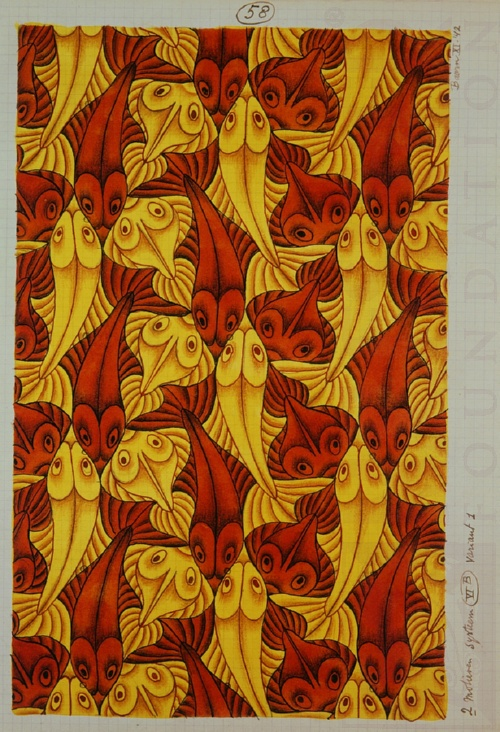
\includegraphics[width=\linewidth]{fig/escher/2-motifs-system.jpg}
	\caption{\href{https://mcescher.com/gallery/symmetry/\#iLightbox[gallery\_image_1]/44}{\emph{2 motifs system VI(b) variant 1}}, M. C. Escher, \textcopyright~The M.C. Escher Company.}
\end{marginfigure}
Given "structures" $\?A_1, \dotsc, \?A_k$ sharing the same "signature",
the $i$-th projection from the Cartesian product $\?A_1 \prodstruct \dotsc \prodstruct \?A_k$
to $\?A_i$, defined by $\tup{a_1,\dotsc,a_k} \mapsto a_i$ ($i \in \intInt{1,k}$),
is a "homomorphism", and is denoted by \AP$\intro*\projHom{i}$.

Given a "$\sigma$-structure" $\?A$, a \AP""congruence@@struct"" on $\?A$
is an equivalence class $\sim$ of $A$ "st" for every
$\+R_{(k)} \in \sigma$, for every $\tup{a_1,\dotsc,a_k} \in \+R(\?A)$,
for any tuple $\tup{a'_1,\dotsc,a'_k} \in A^k$ "st" $a_i \sim a'_i$ for each $i\in \intInt{1,k}$,
then $\tup{a'_1,\dotsc,a'_k} \in \+R(\?A)$.
The \AP""quotient structure"" defined by a "congruence@@struct" $\sim$
on a "structure" $\?A$ has the equivalence classes of $\sim$ as its domain,
and natural "interpretation@@predicates" of the "predicates" and constants.

Given a "homomorphism" $f\colon \?A \to \?B$,
the \AP""congruence induced"" by $f$, and denoted by $\intro*\ker{f}$
is defined by $a \ker{f} a'$ "iff" $f(a) = f(a')$ for all $a, a' \in A$.
It is routine to check that it is indeed a "congruence@@struct" on $\?A$.

We will often implicitly use Noether's first isomorphism theorem:
the "substructure" of $\?B$ "induced@@substructure" by the image $f[A]$
of $A$ is "isomorphic" to the "quotient@@struct" of $\?A$ by $\ker{f}$.

\subsection{Cores}

Two "$\sigma$-structures" $\?A$ and $\?B$ are ""homomorphically equivalent""
if $\?A \homto \?B$ and $\?B \homto \?A$.

A retraction of $\?A$ is a "substructure" $\?A'$ of $\?A$ together with
a "homomorphism" from $\?A$ to $\?A'$ with the property that any vertex of $A'$
is sent on itself.
\begin{proposition}
	Any "finite $\sigma$-structure" $\?A$ admits a unique minimal (in the number of vertices) retraction.
\end{proposition}

\begin{figure}
	\centering
	\begin{tikzpicture}
		\node[vertex, draw=c1, fill=c1, fill opacity=.4] at (0,1) (a) {};
		\node[vertex, draw=c0, fill=c0, fill opacity=.4] at (1.414,1) (b) {};
		\node[vertex, draw=c2, fill=c2, fill opacity=.4] at (2.828,1) (c) {};
		\node[vertex, draw=c1, fill=c1, fill opacity=.4] at (4.242,1) (d) {};
		\node[vertex, draw=c2, fill=c2, fill opacity=.4] at (0.707,0) (e) {};
		\node[vertex, draw=c1, fill=c1, fill opacity=.4] at (2.121,0) (f) {};
		\node[vertex, draw=c3, fill=c3, fill opacity=.4] at (3.536,0) (g) {};
		\node[vertex, draw=c0, fill=c0, fill opacity=.4] at (4.950,0) (h) {};

		\draw[edge] (a) to (b);
		\draw[edge] (b) to (e);
		\draw[edge] (f) to (b);
		\draw[edge] (b) to (c);
		\draw[edge] (f) to (c);
		\draw[edge] (g) to (f);
		\draw[edge] (c) to (g);
		\draw[edge] (d) to (c);
		\draw[edge] (g) to (d);
		\draw[edge] (d) to (h);

		\begin{scope}[xshift=5.5cm]
			\node[vertex, draw=c0, fill=c0, fill opacity=.4] at (1.414,1) (b2) {};
			\node[vertex, draw=c2, fill=c2, fill opacity=.4] at (2.828,1) (c2) {};
			\node[vertex, draw=c1, fill=c1, fill opacity=.4] at (2.121,0) (f2) {};
			\node[vertex, draw=c3, fill=c3, fill opacity=.4] at (3.536,0) (g2) {};

			\draw[edge] (f2) to (b2);
			\draw[edge] (b2) to (c2);
			\draw[edge] (f2) to (c2);
			\draw[edge] (g2) to (f2);
			\draw[edge] (c2) to (g2);
		\end{scope}
	\end{tikzpicture}
	\caption{
		\AP\label{fig:prelim-core}
		On the left-hand side a "graph@@dir", and its "core" on the right.
		The colours are not part of the "structure", but
		are used to describe the retraction of the original
		structure onto its "core".
		(Replica of \Cref{fig:intro-core}.)
	}
\end{figure}
\begin{proof}
	The existence is trivial.
	For the uniqueness, consider two retractions $f_1\colon \?A \homto \?B_1$
	and $f_2\colon \?A \homto \?B_2$. We want to prove that $\?B_1$ and $\?B_2$ are
	"isomorphic".
	Since $\?B_1$ is a "substructure" of $\?A$, consider
	$\restr{f_2}{B_1}\colon \?B_1 \homto \?B_2$. By minimality of $\?B_2$, this "homomorphism"
	must be surjective.
	By symmetry, $\restr{f_1}{B_2}\colon \?B_2 \homto \?B_1$ is also a surjective "homomorphism".
	By composition, we obtain surjective "homomorphism" from $\?B_1$ to itself and from $\?B_2$ to itself. By finiteness, these surjective "homomorphisms" must actually be "automorphisms".
	Hence, it follows that $\restr{f_2}{B_1}$ and $\restr{f_1}{B_2}$ are "isomorphisms",
	and hence $\?B_1$ is "isomorphic" to~$\?B_2$.
\end{proof}

This unique minimal retraction of $\?A$ is called \AP""core"" of $\?A$ and
is denoted by \AP$\intro*\core{\?B}$.
By construction, the "core" of $\?A$ is a "substructure" of $\?A$ to which it is "homomorphically equivalent", see \Cref{fig:prelim-core}.
In general, a \reintro{core} is any "$\sigma$-structure" such that is the "core" of
some "structure"---or equivalently of itself.

\begin{proposition}
	\AP\label{prop:core-iff-hom-are-auto}
	A "finite $\sigma$-structure" $\?C$ is a "core" if, and only if, every
	homomorphism from $\?C$ to itself is an "automorphism".
\end{proposition}

\begin{proof}
	For the left-to-right implication,
	we let $f\colon \?C \to \?C$ be a "homomorphism".
	Then $f[\?C]$ must be "isomorphic" to $\?C$, otherwise we would obtain
	a strictly smaller retraction. Hence, $f$ is a "strong onto homomorphism"
	from $\?C$ to itself, and hence is an "automorphism".
	
	Conversely, assuming that any "homomorphism" from $\?C$ to itself is an "automorphism"
	we get in particular that any retraction must be an "automorphism", and
	hence that $\?C$ is "isomorphic" to $\core{\?C}$.
\end{proof}

\begin{proposition}
	Two "finite structures" are "homomorphically equivalent" if,
	and only if, their "core" are "isomorphic".
\end{proposition}

\begin{proof}
	The right-to-left implication is trivial.
	For the converse one, denote the two "structures" by $\?A_1$ and $\?A_2$,
	and suppose that $\?A_1$ is "homomorphically equivalent" to $\?A_2$.
	Using the "homomorphical equivalence" of $\?A_1$ and $\?A_2$,
	we get retractions of $\?A_2$ onto $\core{\?A}_1$ and of $\?A_1$ onto $\core{\?A}_2$.
	It follows that we have surjective "homomorphisms" from $\core{\?A}_1$ to $\core{\?A}_2$
	and conversely. Hence, $\core{\?A}_1$ and $\core{\?A}_2$ are "isomorphic".
\end{proof}

\begin{proposition}
	\AP\label{prop:adjacency-core}
	Given a "$\sigma$-structure" $\?B$, if $\?B$ is a "core", then
	two elements $b_1$ and $b_2$ of $\?B$ have the same "adjacency" "iff" $b_1 = b_2$.
\end{proposition}

\begin{proof}
	The right-to-left implication is trivial.
	For the converse one, consider the "homomorphism" from $\?B$ to itself
	which maps $b_2$ to $b_1$, and all elements of $B \smallsetminus \{b_2\}$
	to themselves. Since we assumed that $b_1$ and $b_2$ have the same "adjacency",
	this is indeed a "homomorphism", which is clearly not bijective, and
	$\?B$ is not a "core".
\end{proof}

\section{Logic Related Notions}

\subsection{First-Order Logic and Beyond}

We fix a "purely relational signature" $\sigma$.
A (semantical) Boolean \AP""query@@sem"" is any subclass of the
class of all "$\sigma$-structures".
More generally, a $k$-ary \reintro(sem){query} is a function
that maps any "$\sigma$-structure" to a (potentially empty) set of $k$-tuples
of vertices.
We now turn to more syntactical definitions of queries.

We assume that we are given a countable infinite set of variables.
A \AP""first-order formula"" is any formula generated by the grammar 
\[
	\phi {:}{:}= \+R(x_1,\dotsc,x_k) \mid \neg \phi \mid \phi \lor \phi \mid \phi \land \phi
	\mid \exists x.\, \phi \mid \forall x.\, \phi,
\]
where the $x_i$'s ranges over the set of variables and $\+R_{(k)}$ over the "signature" $\sigma$.

\begin{hypothesis}
We assume that, even when not mentioned explicitly, the "signature" contains
a binary "predicate" $=$ that is "interpreted@@predicate" over all "structures"
as equality.
\end{hypothesis}

A \AP""first-order sentence"" is any "first-order formula" with no free variable.
Given a "first-order formula" $\phi$ with free variables $\bar x$, denoted by $\phi(\bar x)$,
and a "pointed $\sigma$-structure" $\tup{\?A,\bar a}$ where the arity of $\bar a$ coincide with
the one of $\bar x$, we denote by $\tup{\?A,\bar a} \intro*\FOmodels \phi(\bar x)$
the fact that $\tup{\?A,\bar a}$ is a model of $\phi(\bar x)$: this can be defined by
a trivial induction on the formula, by interpreting:
\begin{itemize}
	\item the free variable $x_i$ as $a_i$,
	\item the "predicates" $\+R$ as the relation $\+R(\?A)$,
	\item $\neg$, $\lor$, $\land$, $\exists$ and $\forall$ as the Boolean operators of negation, disjunction and conjunction, and as the existential and universal quantifiers, respectively.
\end{itemize}
Given a "$\sigma$-structure" $\?A$, we then denote by \AP$\intro*\semFO{\phi(\bar x)}{\?A}$
the set of tuples $\bar a$ "st" $\tup{\?A, \bar a} \FOmodels \phi(\bar x)$.

We now define the classes $\Pi_n$ and $\Sigma_n$ ($n\in\N$) of "first-order formulas"
as least fixpoints, with the property that $\Sigma_0 \subseteq \Sigma_1 \subseteq \dotsc$ and dually for $\Pi_n$.
We let $\Sigma_0 = \Pi_0$ be the set of quantifier-free formulas.
Then for all $n\in\N$, we consider the following rules:
\[
	\frac{
		\phi \in \Sigma_n
	}{
		\neg \phi \in \Pi_n
	} \qquad\text{and}\qquad
	\frac{
		\phi \in \Pi_n
	}{
		\neg \phi \in \Sigma_n
	},
\]
moreover $\Pi_n \subseteq \Sigma_{n+1}$ and $\Sigma_{n+1}$ is closed under
disjunction, conjunction and existential quantification,
and dually $\Sigma_n \subseteq \Pi_{n+1}$ and $\Pi_{n+1}$ is closed under
disjunction, conjunction and universal quantification.
Formally, the hierarchies
\[
	\Sigma_0 \subseteq \Sigma_1 \subseteq \cdots
	\qquad\text{and}\qquad
	\Pi_0 \subseteq \Pi_1 \subseteq \cdots
\]
are defined as the smallest sets of formulas satisfying these rules.
Then, the \AP""quantifier alternation rank"" of a formula $\phi(\bar x)$
is the least $n\in\N$ "st" $\phi(\bar x)$ belongs to either
$\Sigma_n$ or $\Pi_n$.
Formulas from $\Sigma_1$ are called ""existential formulas"",
those that neither contain negations nor universal quantifications are called \AP""existential-positive formulas"" and lastly, those that neither contain negations
nor any quantifier
are called ""positive quantifier-free formulas"".

A relation over a "$\sigma$-structure" $\?A$ is said to be
\AP""first-order definable"" when it can be written as
$\semFO{\phi(\bar x)}{\?A}$ for some "first-order formula" $\phi(\bar x)$.
Moreover, a class of "$\sigma$-structures" is said to be \reintro{first-order definable},
when there exists a "first-order sentence" $\phi$ "st" the class of "structures" $\?A$
"st" $\?A \FOmodels \phi$ is precisely the class itself.

\AP""First-order logic"" simply consists of the syntax of "first-order formulas" together
with their semantics. Lastly, \AP""monadic second-order logic""
(resp. ""second-order logic"") is obtained from "first-order logic"
by also allowing quantifications over subsets of the structure
(resp. relations of arbitrary arity over the structure).

\subsection{Automata Theory}

Given a set $X$, we denote by $X^*$ and $X^+$ the set of finite words
over $X$, and of non-empty finite words over $X$, respectively.
The empty word is denoted by $\varepsilon$.
An \emph{alphabet} is nothing else but a finite set, and we denote by
$\intro*\2$ the binary alphabet $\{0,1\}$.

In an automaton $\+A$, we denote by \AP $p \intro*\transition{a} q \in \+A$
the fact that there is an $a$-labelled transition from $p$ to $q$.
A \AP""regular language"" is any language---"ie" subset of $\Sigma^*$ for some alphabet $\Sigma$---that
can be recognized by a finite-state automaton.

The signature of words over $\Sigma$ has a binary "predicate" $\preceq$
as well as a unary predicate $a$ for each $a\in \Sigma$.
A word $w_0 \cdots w_{n-1}$ of length $n$
can be seen as a "structure" over the signature of $\Sigma$-words
by taking $\intInt{0,n-1}$ as its domain, "interpreting@@predicate"
$\preceq$ naturally, and interpreting $a\in \Sigma$
as the set of $i \in \intInt{0,n-1}$ "st" $w_i = a$.
It is well-known%
\footnote{See \Cref{sec:preliminaries-automatic-structures-relations-landscape} for details.}
that a language is "regular@@lang" if, and only if, it is definable in "monadic second-order logic".
When $\Sigma = \2$, the signature of $\Sigma$-words is also called 
the \AP""signature of binary strings"".

\subsection{Monoids}

We refer the reader to Pin's seminal lecture notes \cite{Pin2022MathematicalFoundations}
for an introduction to algebraic language theory.

A \AP""monoid"" $\?M = \tup{M,{\cdot},1}$ is a set $M$ together with an associative binary operator $\cdot$ called \emph{product}, and an element $1 \in M$, called \emph{unit}, "st" $x\cdot 1 = x = 1 \cdot x$ for all $x\in M$.
%An \AP""idempotent"" is any element $x\in M$ "st" $x = x^2$.
A \AP""monoid morphism"" is a function between monoids that preserve the product and unit.

"Monoids"---or rather "monoid morphisms"---can be used to recognize languages as $\Sigma^*$
is itself a monoid under concatenation---actually, it is \emph{the free monoid} over $\Sigma$.
A language $L$ is "regular@@lang" if, and only if, there exists a "finite monoid" $\?M$,
and subset $\Acc \subseteq M$ (called \emph{accepting elements}), and a "monoid morphism"
$\phi\colon \Sigma^* \to M$ "st" $L = \phi^{-1}[\Acc]$.
Another way of thinking of the pair $\tup{\phi, M}$ is as follows:
a deterministic complete semiautomaton can be described as a set $Q$ together
with a monoid right action of $\Sigma^*$ over $Q$. On the other hand,
a surjective monoid morphism $\phi\colon \Sigma^* \surj M$ consists of both a monoid
left action and a monoid right action of $\Sigma^*$ over a set $M$,
with the property that $u \cdot (x \cdot v) = (u \cdot x) \cdot v$ for all 
$x\in M$ and $u,v \in \Sigma^*$.
In other words, while automata states represent some information on the word
that is updatable by appending letters on the right, monoid elements represent
an information on the word that is updatable both by appending letters on the left or the right. 

Unsurprisingly, there is a notion of ``minimal information'' required to recognize a monoid,
giving rise to the notions of ""syntactic monoids"" and ""syntactic morphisms"",
see "eg" \cite[Theorem~1.7]{Bojanczyk2020MSO}.

Submonoids and quotient structures are defined analogously to
"substructures" and "quotient structures" for "relational structures".
We say that a "monoid" \AP""divides@@monoid"" another one if it is
a submonoid of one of its quotients.
A \AP""pseudovariety of monoids"" $\symbb{V}$%
consists in a set of "finite monoids" closed under finite Cartesian products
and "monoid division".%
\footnote{``Pseudovariety of \emph{foo}'' and ``variety of finite \emph{foo}''
are used interchangeably in the literature.}
For more details on these,
see \cite[\S XI.1, p.~189]{Pin2022MathematicalFoundations} under the name ``variety''.
On the other hand, a ""$\ast$-pseudovariety of regular languages""
consists of \emph{stream}, "ie" a function $\+V\colon \Sigma \mapsto \+V_{\Sigma}$ from alphabets to languages over this alphabet, with the following properties:%
\footnote{See also \cite[\S XIII.3, p.~226]{Pin2022MathematicalFoundations}.}
\begin{itemize}
	\item it is closed under Boolean operators;
	\item it is closed under preimages by "monoid morphisms", in the sense that
		for every monoid morphism $\phi\colon \Gamma^* \to \Sigma^*$, for any $L \in \+V_{\Sigma}$,
		then $\phi^{—1}[L] \in \+V_{\Gamma}$, and
	\item it is closed under residuals, in the sense that for any $L \in \+V_{\Sigma}$,
		for any $u\in\Sigma^*$, then
		$u^{-1}L \defeq \{v \in \Sigma^* \mid uv \in L\}$
		and $Lu^{-1} \defeq \{v \in \Sigma^* \mid vu \in L\}$
		both belong to $\+V_{\Sigma}$.
\end{itemize}
A seminal result by Eilenberg shows that, mapping a "pseudovariety of monoids" $\symbb{V}$
to the stream associating to $\Sigma$ the set of languages over $\Sigma$ that are recognized
by a "monoid" from $\symbb{V}$ yields a "$*$-pseudovariety of regular languages",
and moreover, this operation is a bijection!
This result generalizes Schützenberger's infamous theorem, showing that
star-free languages are exactly those recognized by aperiodic monoids:
for this reason, this bijection is called the \AP""Eilenberg-Schützenberger correspondence@@lang"".%
\footnote{See \cite[Theorem XIII.4.10, p.~228]{Pin2022MathematicalFoundations} for more details.}

Lastly, given a stream of regular languages $\+V$, the \AP""$\+V$-membership problem@@lang""
takes as input an alphabet $\Sigma$ and a "regular language" $L \subseteq \Sigma^*$,
and asks if $L \in \+V_{\Sigma}$. When $\+V$ is a "pseudovariety of regular languages",
a powerful technique to solve this problem is to prove that the membership problem
of the "corresponding@@EilenbergLang" "pseudovariety of monoids" is decidable.

\todo{move apdx here}

\section{Computability and Complexity}

\subsection{Turing Machines}

\marginnote{\blockquote[Gilles Dowek, Laurence Devillers \& Serge Abiteboul, \emph{Qui a hacké Garoutzia}]{Mais dans ce sandwich absurde entre mon initialisation et ma terminaison, que m'aura-t-il vraiment manqué ? Peut-être un corps… un corps qui ressent et tutti quanti !}}
We assume that the reader is familiar with Turing machines,
see "eg" \cite[\S~1]{AroraBarak2009ComputationalComplexity}.
Unless stated otherwise, a \AP""Turing machine"" is assumed to have a single tape,
which is bounded on the left but not on the right.
The ""configuration@@TM"" of a "Turing machine" consists of
the content of the tape at a given point, the position of the machine's head,
at well as its current state. It can be summarized by
a triple $\tup{u, q, v}$, where $q$ denotes the current state,
$u$ is the word written strictly on the left of the head,
and $v$ is the word written to the right of the head (head included).
The \AP""initial configuration"" of a "Turing machine" $\+M$ refers to the "configuration@@TM" 
$\tup{\varepsilon, q_0, \varepsilon}$ where $q_0$ is the initial state of $\+M$.
A "configuration@@TM" is \AP""reachable@@configuration"" whenever
it can be obtained from the "initial configurations" by applying a finite sequence
of transitions of the machine.

\subsection{Elements of Complexity Theory}

We assume familiarity with basic complexity classes, see "eg"
\cite[\S\!\S~2--5]{AroraBarak2009ComputationalComplexity}.
We say that two decision problems are \AP""computationally equivalent""
when there are many-one reductions between them.

% REPLACE NEXT PARAGRAPH WITH: WHEN FIGURE WILL BE DONE.
% In the following hierarchy, we
% describe the different complexity classes that appear in this document:
% those appearing in bold play a `crucial role' in this thesis and are briefly defined
% in this document; the other ones---they are often only mentioned when talking about
% the literature---point to the "Complexity Zoo".
% We also mention a few decisions problems studied in this thesis---they will be introduced
% as needed.

\paragraph*{Complexity Classes.}
Here are the most important classes that appear in this document---the other ones
will all point to their respective entry in the "Complexity Zoo":
\begin{itemize}
	\item "FOfin" refers to "first-order definable classes", see \Cref{sec:prelim-auto-FO} for the definition;
	\itemAP ""L"" and ""NL"" refer to problems solvable in deterministic and non-deterministic logarithmic 
	space; for hardness we usually consider "first-order reductions";
	\itemAP ""P"" (resp. ""PSpace"") refers to problems solvable in deterministic polynomial time
	(resp. polyomial space); hardness is usually considered under logarithmic-space reductions;
	\itemAP ""NP"" and ""coNP"" refer to the first level of the polynomial-time hierarchy
		\cite[\S~2]{AroraBarak2009ComputationalComplexity},
		and ""SigmaP2"", ""PiP2"" to its second level,
		see "eg" \cite[\S~5]{AroraBarak2009ComputationalComplexity};
		hardness is usually considered under logarithmic-space reductions;
	\itemAP ""$k$-ExpTime"" and ""$k$-ExpSpace"" are the
		problems solvable in time and space
		\[n \mapsto \underbrace{2^{2^{{\,\rotatebox{90}{\tiny$\ddots$}\,}^{2^{\textrm{poly}(n)}}}}}_{k \text{ times}},\]
		respectively; hardness is considered under polynomial-time reductions;
	\itemAP ""Tower"" is the class of problems that can be solved in time
		$n\mapsto \tower(f(n))$ for some elementary function $f$,%
		\footnote{Recall that an function is said to be elementary when it
		is bounded by a tower of exponentials of fixed height.}
		where $\intro*\tower(n) \defeq t(n,n)$ and $t$ is the function
		defined recursively by $t(p,q) \defeq 2^{t(p-1,q)}$ and $t(0,q) \defeq q$:
		in other words $\tower(n)$ it is a tower of exponentials whose height is given by the input;
		hardness is defined under elementary reductions,
		see \cite{Schmitz2016ComplexityHierarchies} for more details on this class.
\end{itemize}

\paragraph*{Computability Classes.}
We now turn to undecidable classes: all hardness result are considered up to
many-one reductions, "ie" instance-preserving computable functions.
We denote by \AP""RE"" and ""coRE"" the classes of recursively enumerable
and co-recursively enumerable problems, respectively. 
The next levels $\Sigma^0_n$ and $\Pi^0_n$ of the \AP""arithmetical hierarchy"" can be defined 
as the classes of sets that are "definable@@first-order" by a "first-order formula"
from the fragments $\Sigma_n$ and $\Pi_n$, respectively, in the structure $\tup{\N,+,\cdot}$.
It can be shown that $\Sigma^0_0 = \Pi^0_0$ corresponds to the class of all decidable problems,
and $\Sigma^0_1 =$ "RE" and $\Pi^0_1$ = "coRE". The only other levels that will be of interest
to us will be \AP""Sigma0-2"" and ""Pi0-2"".
The ""analytical hierarchy"" is defined analogously, by replacing "first-order logic" with
"second-order logic".


\paragraph*{Decision Problems.}
\AP""Connectivity in Finite Graphs"" is the decision problem
that takes as input a "graph@@dir" and two vertices $s$ and $t$,
and asks if they are "connected".
\AP ""Reachability in Finite Graphs"" is defined analogously,
but asks rather if there is a directed path from $s$ to $t$.
Surprisingly, despite their resemblance, these two problems have a distinct complexity:
"Reachability in finite graphs" is "NL"-complete, see "eg"
\cite[Theorem~4.18]{AroraBarak2009ComputationalComplexity}, while "Connectivity in finite graphs"
is only in "L" by Reingold's theorem, see "eg"
\cite[Theorem~21.21]{AroraBarak2009ComputationalComplexity}.
In fact, the problem is "L"-complete:
Etessami even proved that the problem
was "L"-hard under "first-order reductions" even if the "graph@@dir" is restricted to
be a "directed path@$k$-path" \cite[Theorem 3.2]{Etessami1997CountingLogSpace}!